\documentclass[11pt]{article}
\usepackage{amssymb,amsmath}
\usepackage{mathrsfs}  
\usepackage{graphicx}
\usepackage[margin=2cm]{geometry}
\usepackage{tikz}
\usepackage{soul}
\usepackage{xfrac}
\usepackage[tikz]{mdframed}
\mdfdefinestyle{hlframe}{%      
frametitlebackgroundcolor   =black!15,%                                    
    backgroundcolor   =black!5,%                                               
    frametitlerule          =true,%                                            
    roundcorner     =10pt,%                                                
    middlelinewidth     =1pt,%                                             
    innermargin     =0.5cm,%                                               
    outermargin     =0.5cm,%                                               
    innerleftmargin     =0.5cm,%                                           
    innerrightmargin        =0.5cm,%                                       
    innertopmargin      =0.75\topskip,%                                    
    innerbottommargin   =0.75\topskip,%                                    
}
\usepackage{hyperref}
\hypersetup{
    colorlinks=true,
    linkcolor=blue,
    citecolor=red,
    filecolor=magenta,      
    urlcolor=blue
    }
\usepackage{algorithm}
\usepackage{algpseudocode}
\renewcommand{\div}{\textsf{div}}
\newcommand{\grad}{\textsf{grad}}
\newcommand{\rot}{\textsf{rot}}
\newcommand{\cellint}[2]{\Big(#1\Big)_{#2}}
\newcommand{\cellintK}[1]{\cellint{#1}{K}}
\newcommand{\facetint}[2]{\Big\langle #1\Big\rangle_{#2}}
\newcommand{\facetintK}[1]{\facetint{#1}{\partial K}}
\newcommand{\facetinttime}[3]{\Big\langle\!\!\Big\langle #1\Big\rangle\!\!\Big\rangle_{#2}^{t=#3}}
\newcommand{\facetinttimeK}[2]{\Big\langle\!\!\Big\langle #1\Big\rangle\!\!\Big\rangle_{K}^{t=#2}}
\newcommand{\phat}{\widehat{p}}
\newcommand{\jump}[1]{[\![ #1]\!]}
\newcommand{\avg}[1]{\{\!\{#1\}\!\}}
\renewcommand{\vec}[1]{\boldsymbol{#1}}
\newcommand{\dof}[1]{\vec{#1}}
\newcommand{\fspace}[1]{\mathscr{#1}}
\newcommand{\spaceV}{\fspace{V}}
\newcommand{\spaceT}{\fspace{T}}
\newcommand{\pref}{p_{\text{ref}}}
\newcommand{\Id}{\operatorname{Id}}
\newcommand{\impl}{{(\text{im})}}
\newcommand{\expl}{{(\text{ex})}}
\title{IMEX-HDG dicsretisation of incompressible Euler equations}
\date{\today}
\begin{document}
\maketitle
The goal of this note is to derive a hybridisable discontinuous Galerkin (HDG) projection method \cite{Chorin1968} for the time-dependent incompressible Euler equation, similar to \cite{Ueckermann2016} where this approach is applied to the Navier-Stokes equations. While in \cite{Ueckermann2016} the presence of the Stokes term requires the hybridisation of both the tentative velocity computation and the pressure solve, for the incompressible Euler equations this is only required in the latter step. The starting point of our derivation is the fully implicit DG formulation of the incompressible Euler equations in \cite{Guzman2016}. Similar to \cite{Ueckermann2016}, we also discuss higher-order IMEX timestepping methods \cite{Ascher1997}. To solve the resulting mixed pressure equation we use a Schur-complement approach and the non-nested multigrid preconditioner described in \cite{Cockburn2014}.
%%%%%%%%%%%%%%%%%%%%%%%%%%%%%%%%%%%%%%%%%%%%%%%%%%%%%%%%%%%%%%%%%%%%%%%%%%%%%%%%%%%%%%%%%%%
\section{Continuum equations}
%%%%%%%%%%%%%%%%%%%%%%%%%%%%%%%%%%%%%%%%%%%%%%%%%%%%%%%%%%%%%%%%%%%%%%%%%%%%%%%%%%%%%%%%%%%
We consider the incompressible Euler equations for velocity $Q(x,t)$ and pressure $p(x,t)$
\begin{equation}
    \begin{aligned}
        \partial_t Q + (Q\cdot \nabla) Q + \nabla p & = f \\
        \nabla\cdot Q                               & = 0
    \end{aligned}\label{eqn:incompressible_euler}
\end{equation}
in the domain $\Omega=[0,1]^d$ with the initial condition $Q(x,0) = Q_0(x)$ and the boundary condition \mbox{$n\cdot Q\vert_{\partial \Omega}=0$} on $\partial\Omega$. $f$ is a time dependent forcing function.
%%%%%%%%%%%%%%%%%%%%%%%%%%%%%%%%%%%%%%%%%%%%%%%%%%%%%%%%%%%%%%%%%%%%%%%%%%%%%%%%%%%%%%%%%%%
\section{Notation}
%%%%%%%%%%%%%%%%%%%%%%%%%%%%%%%%%%%%%%%%%%%%%%%%%%%%%%%%%%%%%%%%%%%%%%%%%%%%%%%%%%%%%%%%%%%
We write $\Omega_h$ for the mesh and $\mathcal{E}_h$ for the skeleton of this mesh, i.e. the set of all facets. The set of interior facets is denoted by $\mathcal{E}^i_h$ and the set of boundary facets by $\mathcal{E}^\partial_h$ such that $\mathcal{E}_h= \mathcal{E}^i_h\cup \mathcal{E}^\partial_h$ . Further, for scalar quantities $a$ and vector-valued quantities $b$ we define the average $\avg{\cdot}$ and jump $\jump{\cdot}$ as
\begin{xalignat}{3}
    \avg{a} &:= \frac{1}{2}(a^++a^-), &
    \avg{b} &:= \frac{1}{2}(b^++b^-), &
    \jump{b\cdot n} &:= b^+\cdot n^+ + b^-\cdot n^-
\end{xalignat}
on interior facets $F\in\mathcal{E}_h^i$ and
\begin{xalignat}{3}
    \avg{a} &:= a, &
    \avg{b} &:= b, &
    \jump{b\cdot n} &:= b\cdot n
\end{xalignat}
on boundary facets $F\in\mathcal{E}_h^\partial$. The inner product of two tensors $A$, $B$ is
\begin{equation}
    A:B := \sum_{ij} A_{ij} B_{ji} = \operatorname{trace}(AB^\top).
\end{equation}
We use the shorthand
\begin{equation}
    (f)_A = \int_A f\;dx\qquad\text{for $A \subset \Omega$}
\end{equation}
for integrals over $d$-dimensional domains $A$ (typically grid cells) and
\begin{equation}
    \langle f\rangle_S = \int_S f\;ds\qquad\text{for $S \subset \mathcal{E}_h$}
\end{equation}
for integrals over $d-1$-dimensional domains (typically facets, boundaries of grid cells).
%%%%%%%%%%%%%%%%%%%%%%%%%%%%%%%%%%%%%%%%%%%%%%%%%%%%%%%%%%%%%%%%%%%%%%%%%%%%%%%%%%%%%%%%%%%
\section{DG discretisation}
%%%%%%%%%%%%%%%%%%%%%%%%%%%%%%%%%%%%%%%%%%%%%%%%%%%%%%%%%%%%%%%%%%%%%%%%%%%%%%%%%%%%%%%%%%%
We follow the DG discretisation with a central flux as described in \cite{Guzman2016}. Let $P_k(A)$ be the space of polynomials of degree $k$ on $A$, then we define the DG space as
\begin{equation}
    \text{DG}_k := \{ v\in L^2(\Omega) : v|_K \in P_k(K) \;\text{for all}\;K\in \Omega_h \}
\end{equation}
and assume that
\begin{equation}
    \begin{aligned}
        Q \in V_Q & := [\text{DG}_{k+1}]^d,                    \\
        p \in Q_p & := \text{DG}_{k}\cap \{v:(v)_{\Omega}=0\}. \\
    \end{aligned}\label{eqn:function_spaces}
\end{equation}
We start by post-processing the velocity $Q$ into the divergence free advection velocity $Q^\star$ which is defined as follows:
%%%%%%%%%%%%%%%%%%%%%%%%%%%%%%%%%%%%%%%%%%%%%%%%%%%%%%%%%%%%%%%%%%%%%%%%%%%%%%%%%%%%%%%%%%%
\subsection{Post-processed advection velocity}
%%%%%%%%%%%%%%%%%%%%%%%%%%%%%%%%%%%%%%%%%%%%%%%%%%%%%%%%%%%%%%%%%%%%%%%%%%%%%%%%%%%%%%%%%%%
Let $\text{ND}_{k-1}(K)$ be the space of Nedelec functions of the first kind \cite[Section 3.5.1]{Logg2012}\footnote{Note that in \cite{Logg2012} the lowest order Nedelec element is $\text{ND}_{1}(K)$ whereas it is $\text{ND}_{0}(K)$ in \cite{Guzman2016}; here we use the counting employed in \cite{Guzman2016}.} on the cell $K$. In each cell $K\in\Omega_h$ and for a given $Q\in V_Q$ we look for $(Q^\star_K,\sigma_K,r_K) \in W_K = [P_{k+1}(K)]^d\times \text{ND}_{k-1}(K)\times \left(\oplus_{F\in\partial K} P_{k+1}(F)\right)$ which satisfy the following weak form:
\begin{equation}
    (Q^\star_K\cdot  \omega_K)_K + \langle (Q_K^\star\cdot n)s_K\rangle_{\partial K} + (v_K\cdot \sigma_K)_K + \langle (v_K\cdot n)r_K\rangle_{\partial K} = (Q\cdot\omega_K)_K + \langle (Q\cdot n)s_K\rangle_{\partial K\cap \mathcal{E}_h^i}\label{eqn:bdm_projection}
\end{equation}
for all test functions $(v_K,\omega_K,s_K)\in W_K$. Note that since the solution satisfies $\sigma_K=0$ and $r_K=0$ this is equivalent to Eqs. (2.25) and (2.26) in \cite{Guzman2016}, but to implement these two constraints in Firedrake we need to make sure that the weak form corresponds to a square matrix. For future reference we write $Q^\star = \mathcal{P}(Q)$, observing that $\mathcal{P}:V_Q \rightarrow V_Q$ is a linear operator; in fact as argued in \cite{Guzman2016} $\mathcal{P}$ projects onto the H-div conforming subspace $\text{BDM}^0_{k+1}(\Omega_h)$. The normal component of $Q^\star$ is continuous ($\jump{Q^\star\cdot n} = 0$). Since we only consider integrals over interior facets in the final term on the right hand side of Eq. \eqref{eqn:bdm_projection}, we have that $(n\cdot Q^\star)_{\partial \Omega} = 0$ on the boundary $\partial\Omega$ of the domain. As shown in \cite{Guzman2016} the post-processed velocity $Q^\star$ is divergence free in the strong sense $\nabla \cdot Q^\star=0$.
%%%%%%%%%%%%%%%%%%%%%%%%%%%%%%%%%%%%%%%%%%%%%%%%%%%%%%%%%%%%%%%%%%%%%%%%%%%%%%%%%%%%%%%%%%%
\subsection{Original scheme}
%%%%%%%%%%%%%%%%%%%%%%%%%%%%%%%%%%%%%%%%%%%%%%%%%%%%%%%%%%%%%%%%%%%%%%%%%%%%%%%%%%%%%%%%%%%
The discretisation proposed in \cite{Guzman2016} (see Eqs. (2.27) and (2.28) there) is: for given forcing function $f$ find $(Q,p)\in V_Q\times V_p$ such that
\begin{equation}
    \begin{aligned}
        (\partial_t Q\cdot w)_{K} - (Q\otimes Q^\star:\nabla w)_{K} - (p\nabla\cdot w)_{K} + \langle \widehat{\sigma}: n\otimes w \rangle_{\partial K} & = (f\cdot w)_{K} \\
        - (Q\cdot \nabla \psi)_{K} + \langle (\widehat{Q}\cdot n)\psi\rangle_{\partial K}                                                              & =0
    \end{aligned}
\end{equation}
for all test functions $(w,\psi)\in V_Q\times V_p$ and all cells. The numerical fluxes $\widehat{\sigma}$ and $\widehat{Q}$ are defined as
\begin{equation}
    \begin{aligned}
        \widehat{\sigma}   & := \avg{p} \Id  + \alpha h_F^{-1} \jump{Q\cdot n} \Id       + \begin{cases}
                                                                                               \avg{Q}\otimes Q^\star       & \text{for the central flux}, \\
                                                                                               Q^{\text{up}}\otimes Q^\star & \text{for the upwind flux}
                                                                                           \end{cases} \\
        \widehat{Q}\cdot n & := \avg{Q}\cdot n.
    \end{aligned}\label{eqn:flux_original}
\end{equation}
with the upwind velocity defined as
\begin{equation}
    Q^\text{up} = \begin{cases}
        Q^+ & \text{if $Q\cdot n\ge 0$} \\
        Q^- & \text{otherwise}
    \end{cases}
\end{equation}
This leads to the time-dependent scheme for computing $(Q^{n+1},p^{n+1})\in V_Q\times V_p$ from $Q^n$ and $f^n$, the value of the forcing function at timestep $n$:
\begin{subequations}
    \begin{align}
        (Q^{n+1}\cdot w)_{\Omega_h} + \Delta t\Big[  \left(w\cdot (Q^\star\cdot \nabla) Q^{n+1}\right)_{\Omega_h}                                                                                            &
        \notag                                                                                                                                                                                                                                                                     \\ + \alpha \Big(\sum_{F\in\mathcal{E}_h^i} h_F^{-1}\langle \jump{Q^{n+1}\cdot n} \jump{w\cdot n}\rangle_F                                      +  \sum_{F\in\mathcal{E}_h^\partial} h_F^{-1}\langle (Q^{n+1}\cdot n) (w\cdot n)\rangle_F \Big)                                        &  \label{eqn:time_dependent_original_momentum}                                                            \\
        -\sum_{F\in\mathcal{E}_h^i} \langle (Q^\star \cdot n^+)(Q^{n+1}_+ - Q^{n+1}_-)\cdot \avg{w}\rangle_F\notag                                                                                           &                                                                     \\
        +\delta_{\text{up}}\sum_{F\in\mathcal{E}_h^i} \langle \left|Q^\star \cdot n^+\right|(Q^{n+1}_+ - Q^{n+1}_-)\cdot (w^+-w^-)\rangle_F
                                                                                                                                                                                                             & \notag                                                              \\
        - (p^{n+1} \nabla\cdot w)_{\Omega_h} +  \sum_{F\in\mathcal{E}_h^i} \langle \jump{w\cdot n}\avg{p^{n+1}}\rangle_{F}+  \sum_{F\in\mathcal{E}_h^\partial} \langle (w\cdot n)p^{n+1}\rangle_{F}    \Big] & = (Q^n\cdot w)_{\Omega_h} + \Delta t (f^n\cdot w)_{\Omega_h} \notag \\
        (\psi \nabla\cdot Q^{n+1})_{\Omega_h} - \sum_{F\in\mathcal{E}_h^i} \langle \jump{Q^{n+1}\cdot n}\avg{\psi}\rangle_{F} - \sum_{F\in\mathcal{E}_h^\partial} \langle (Q^{n+1}\cdot n)\psi\rangle_{F}    & = 0\label{eqn:time_dependent_original_continuity}
    \end{align}
\end{subequations}
for all test functions $(w,\psi) \in V_Q\times V_p$ where $\delta_{\text{up}}=1$ for the upwind flux and $\delta_{\text{up}}=0$ for the central flux. In contrast to \cite{Guzman2016} the boundary condition $(n\cdot Q^{n+1})_{\partial \Omega}=0$ is enforced weakly through the penalty term in the second line of Eq. \eqref{eqn:time_dependent_original_momentum}, this introduces additional boundary integrals.
%%%%%%%%%%%%%%%%%%%%%%%%%%%%%%%%%%%%%%%%%%%%%%%%%%%%%%%%%%%%%%%%%%%%%%%%%%%%%%%%%%%%%%%%%%%
\subsection{Hybridised scheme}\label{sec:hdg_implicit}
%%%%%%%%%%%%%%%%%%%%%%%%%%%%%%%%%%%%%%%%%%%%%%%%%%%%%%%%%%%%%%%%%%%%%%%%%%%%%%%%%%%%%%%%%%%
To hybridise we replace the numerical fluxes in Eq. \eqref{eqn:flux_original} by
\begin{equation}
    \begin{aligned}
        \widehat{\sigma}   & := \lambda \Id  + \alpha h_F^{-1} \jump{Q\cdot n} \Id       + \begin{cases}
                                                                                               \avg{Q}\otimes Q^\star       & \text{for the central flux}, \\
                                                                                               Q^{\text{up}}\otimes Q^\star & \text{for the upwind flux}
                                                                                           \end{cases} \\
        \widehat{Q}\cdot n & := Q\cdot n + \tau (p-\lambda).
    \end{aligned}\label{eqn:flux_hdg}
\end{equation}
for some stability parameter $\tau>0$ and the function $\lambda\in V_\text{trace}$ defined on the trace space
\begin{equation}
    V_{\text{trace}} = \{ v\in L^2(\mathcal{E}_h) : v|_F \in P_k(F) \;\text{for all}\;F\in \mathcal{E}_h \}.
\end{equation}
We also introduce a transmission condition which guarantees that the normal component of $\widehat{Q}$ is single-valued:
\begin{equation}
    0 = \langle \jump{\widehat{Q}\cdot n} \mu \rangle_F = \langle (\jump{Q\cdot n} + 2\tau\avg{p-\lambda})\mu \rangle_F \qquad \text{for all $F\in\mathcal{E}_h^i$ and all $\mu\in V_{\text{trace}}$} \label{eqn:jump_condition_interior}
\end{equation}
and enforce the boundary condition weakly by requiring that
\begin{equation}
    0 = \langle (\widehat{Q}\cdot n) \mu \rangle_F = \langle (Q\cdot n + \tau(p-\lambda))\mu \rangle_F \qquad \text{for all $F\in\mathcal{E}_h^\partial$ and all $\mu\in V_{\text{trace}}$}\label{eqn:jump_condition_boundary}
\end{equation}
As a result, Eqs. \eqref{eqn:time_dependent_original_momentum} and \eqref{eqn:time_dependent_original_momentum} get replaced by: for given $Q^n,f^n\in V_Q$ find
$(Q^{n+1},p^{n+1},\lambda^{n+1})\in V_Q\times V_p\times V_{\text{trace}}$
\begin{subequations}
    \begin{align}
        (Q^{n+1}\cdot w)_{\Omega_h} + \Delta t\Big[  \left(w\cdot (Q^\star\cdot \nabla) Q^{n+1}\right)_{\Omega_h}  -\sum_{F\in\mathcal{E}_h^i} \langle (Q^\star \cdot n^+)(Q^{n+1}_+ - Q^{n+1}_-)\cdot \avg{w}\rangle_F                              &
        \notag                                                                                                                                                                                                                                                                                                             \\
        +\delta_{\text{up}}\sum_{F\in\mathcal{E}_h^i} \langle \left|Q^\star \cdot n^+\right|(Q^{n+1}_+ - Q^{n+1}_-)\cdot (w^+-w^-)\rangle_F                                                                                                          & \label{eqn:time_dependent_hdg_momentum}                             \\
        + \alpha \Big(\sum_{F\in\mathcal{E}_h^i} h_F^{-1}\langle \jump{Q^{n+1}\cdot n} \jump{w\cdot n}\rangle_F                                      +  \sum_{F\in\mathcal{E}_h^\partial} h_F^{-1}\langle (Q^{n+1}\cdot n) (w\cdot n)\rangle_F \Big) & \notag                                                              \\
        - (p^{n+1} \nabla\cdot w)_{\Omega_h} +  \sum_{F\in\mathcal{E}_h^i} \langle \jump{w\cdot n}\lambda^{n+1}\rangle_{F}  +  \sum_{F\in\mathcal{E}_h^\partial} \langle (w\cdot n)\lambda^{n+1}\rangle_{F}     \Big]                                & = (Q^n\cdot w)_{\Omega_h} + \Delta t (f^n\cdot w)_{\Omega_h} \notag \\
        (\psi \nabla\cdot Q^{n+1})_{\Omega_h} + 2 \sum_{F\in\mathcal{E}_h^i} \langle \avg{\tau (p^{n+1}-\lambda^{n+1})\psi}\rangle_{F}            + \sum_{F\in\mathcal{E}_h^\partial} \langle \tau (p^{n+1}-\lambda^{n+1})\psi\rangle_{F}            & = 0  \label{eqn:time_dependent_hdg_continuity}                      \\
        \sum_{F\in\mathcal{E}_h^i} \langle \left(\jump{Q^{n+1}\cdot n}+2\tau \avg{p^{n+1}-\lambda^{n+1}}\right)\mu \rangle_{F} + \sum_{F\in\mathcal{E}_h^\partial} \langle \left(Q^{n+1}\cdot n+\tau (p^{n+1}-\lambda^{n+1})\right)\mu \rangle_{F}   & = 0\label{eqn:time_dependent_hdg_trace}
    \end{align}
\end{subequations}
for all test functions $(w,\psi,\mu) \in V_Q\times V_p\times V_{\text{trace}}$. Observe that Eqs. \eqref{eqn:time_dependent_original_momentum} and \eqref{eqn:time_dependent_hdg_momentum} only differ in the final two terms on the left hand side.
%%%%%%%%%%%%%%%%%%%%%%%%%%%%%%%%%%%%%%%%%%%%%%%%%%%%%%%%%%%%%%%%%%%%%%%%%%%%%%%%%%%%%%%%%%%
\subsection{Split hybridised scheme}\label{sec:split_hybridised}
%%%%%%%%%%%%%%%%%%%%%%%%%%%%%%%%%%%%%%%%%%%%%%%%%%%%%%%%%%%%%%%%%%%%%%%%%%%%%%%%%%%%%%%%%%%
Finally, we split the update $Q^{n} \mapsto (Q^{n+1},p^{n+1},\lambda^{n+1})$ in Eqs. \eqref{eqn:time_dependent_hdg_momentum}, \eqref{eqn:time_dependent_hdg_continuity}, \eqref{eqn:time_dependent_hdg_trace} into two steps:
\begin{itemize}
    \item The computation of a tentative velocity $\overline{Q}$ which is not necessarily divergence-free
    \item The solution of a mixed Poisson equation for the pressure $p^{n+1}$ at the next time step and a velocity correction $\delta Q$ which renders the velocity $Q^{n+1} = \overline{Q}-\Delta t \delta Q$ at the next timestep divergence free (in the weak sense)
\end{itemize}
%%%%%%%%%%%%%%%%%%%%%%%%%%%%%%%%%%%%%%%%%%%%%%%%%%%%%%%%%%%%%%%%%%%%%%%%%%%%%%%%%%%%%%%%%%%
\paragraph{Tentative velocity.}
%%%%%%%%%%%%%%%%%%%%%%%%%%%%%%%%%%%%%%%%%%%%%%%%%%%%%%%%%%%%%%%%%%%%%%%%%%%%%%%%%%%%%%%%%%%
To obtain $\overline{Q}$, replace $Q^{n+1} \mapsto \overline{Q}$ in Eq. \eqref{eqn:time_dependent_hdg_momentum} and drop all terms which contain the pressure $p^{n+1}$ and hybridised pressure $\lambda^{n+1}$ (these will be dealt with in the next step):
\begin{equation}
    \begin{aligned}
        (\overline{Q}\cdot w)_{\Omega_h} + \Delta t\Big[  \left(w\cdot (Q^\star\cdot \nabla) \overline{Q}\right)_{\Omega_h}  -\sum_{F\in\mathcal{E}_h^i} \langle (Q^\star \cdot n^+)(\overline{Q}_+ - \overline{Q}_-)\cdot \avg{w}\rangle_F & \\
        +\delta_{\text{up}}\sum_{F\in\mathcal{E}_h^i} \langle \left|Q^\star \cdot n^+\right|(\overline{Q}_+ - \overline{Q}_-)\cdot (w^+-w^-)\rangle_F                                                                                       & \\+ \alpha \Big(\sum_{F\in\mathcal{E}_h^i} h_F^{-1}\langle \jump{\overline{Q}\cdot n} \jump{w\cdot n}\rangle_F                                      +  \sum_{F\in\mathcal{E}_h^\partial} h_F^{-1}\langle (\overline{Q}\cdot n) (w\cdot n)\rangle_F \Big)  \Big]          & = (Q^n\cdot w)_{\Omega_h} + \Delta t (f^n\cdot w)_{\Omega_h}
    \end{aligned}\label{eqn:tentative_velocity}
\end{equation}
%%%%%%%%%%%%%%%%%%%%%%%%%%%%%%%%%%%%%%%%%%%%%%%%%%%%%%%%%%%%%%%%%%%%%%%%%%%%%%%%%%%%%%%%%%%
\paragraph{Mixed Poisson.}
%%%%%%%%%%%%%%%%%%%%%%%%%%%%%%%%%%%%%%%%%%%%%%%%%%%%%%%%%%%%%%%%%%%%%%%%%%%%%%%%%%%%%%%%%%%
In the continuum, the mixed Poisson equation that we need to solve can be written as
\begin{xalignat}{2}
    \delta Q + \nabla p^{n+1} &= 0, &
    \nabla \cdot \delta Q &= -\frac{1}{\Delta t} \nabla\cdot \overline{Q}.\label{eqn:mixed_poisson_continuum}
\end{xalignat}
In a single cell $K$ the weak form is
\begin{equation}
    \begin{aligned}
        (w\cdot \delta Q)_K - (p^{n+1} \nabla \cdot w)_K + \langle(n\cdot w) \widehat{p}^{n+1}\rangle_{\partial K}   & = 0,                                                                                                                                                 \\
        (\psi \nabla \cdot\delta Q)_K + \langle \psi(\widehat{\delta Q}\cdot n- \delta Q\cdot n)\rangle_{\partial K} & = -\frac{1}{\Delta t}\left((\psi\nabla\cdot\overline{Q})_K - \langle \psi(\overline{Q}-\mathcal{A}(\overline{Q}))\cdot n\rangle_{\partial K} \right)
    \end{aligned}
\end{equation}
with the hybridised fluxes
\begin{equation}
    \begin{aligned}
        \widehat{p}^{n+1}         & = \lambda^{n+1}                                 \\
        \widehat{\delta Q}\cdot n & = \delta Q\cdot n + \tau(p^{n+1}-\lambda^{n+1})
    \end{aligned}
\end{equation}
where $\tau$ is the stabilisation parameter as before.
The velocity $\mathcal{A}(\overline{Q})$ is single valued on each facet and defined as
\begin{equation}
    \mathcal{A}(Q) := \begin{cases}
        0       & \text{on boundary facets $F \subset \partial \Omega$ }  \\
        \avg{Q} & \text{on interior facets $F\not\subset\partial\Omega$.} \\
    \end{cases}.
\end{equation}
We also require the numerical flux $\widehat{\delta Q}$ to be unique on interior facets and enforce the flux boundary condition $(Q\cdot n)_{\partial \Omega}=0$ weakly:
\begin{equation}
    \begin{aligned}
        \langle \jump{\widehat{\delta Q}\cdot n} \mu \rangle_F = \langle (\jump{\delta Q\cdot n} + 2\tau\avg{p^{n+1}-\lambda^{n+1}})\mu \rangle_F & =0 \qquad \text{for all $F\in\mathcal{E}_h^i$}         \\
        \langle (\widehat{\delta Q}\cdot n) \mu \rangle_F = \langle (\delta Q\cdot n + \tau(p^{n+1}-\lambda^{n+1}))\mu \rangle_F                  & = 0\qquad \text{for all $F\in\mathcal{E}_h^\partial$}.
    \end{aligned}
\end{equation}
for all test functions $\mu\in V_{\text{trace}}$.
Putting everything together we need to solve the following weak problem: find $(\delta Q,p^{n+1},\lambda^{n+1}) \in V_Q\times V_p\times V_{\text{trace}}$ such that
\begin{subequations}
    \begin{align}
        (\delta Q\cdot w)_{\Omega_h} - (p^{n+1} \nabla\cdot w)_{\Omega_h} +  \sum_{F\in\mathcal{E}_h^i} \langle \jump{w\cdot n}\lambda^{n+1}\rangle_{F}  +  \sum_{F\in\mathcal{E}_h^\partial} \langle (w\cdot n)\lambda^{n+1}\rangle_{F}             & = 0\label{eqn:mixed_poisson_velocity}                                                   \\
        (\psi \nabla\cdot \delta Q)_{\Omega_h} + 2 \sum_{F\in\mathcal{E}_h^i} \langle \avg{\tau (p^{n+1}-\lambda^{n+1})\psi}\rangle_{F}            + \sum_{F\in\mathcal{E}_h^\partial} \langle \tau (p^{n+1} - \lambda^{n+1})\psi\rangle_{F}         & = -\frac{1}{\Delta t}  \text{Div}(\psi,\overline{Q}) \label{eqn:mixed_poisson_pressure} \\
        \sum_{F\in\mathcal{E}_h^i} \langle \left(\jump{\delta Q\cdot n}+2\tau \avg{p^{n+1}-\lambda^{n+1}}\right)\mu \rangle_{F} + \sum_{F\in\mathcal{E}_h^\partial} \langle \left(\delta Q\cdot n+\tau (p^{n+1}-\lambda^{n+1})\right)\mu \rangle_{F} & = 0
        \label{eqn:mixed_poisson_uniqueness}
    \end{align}
\end{subequations}
for all test functions $(w,\psi,\mu) \in V_Q\times V_p\times V_{\text{trace}}$ where the weak divergence is given by
\begin{equation}
    \text{Div}(\psi,Q) := (\psi \nabla \cdot Q)_{\Omega_h}-2\sum_{F\in\mathcal{E}_h^i}\langle(\avg{\psi Q}-\avg{\psi}\avg{Q})\cdot n\rangle_F-\sum_{F\in\mathcal{E}_h^\partial}\langle\psi (Q\cdot n)\rangle_F.\label{eqn:weak_divergence}
\end{equation}
%%%%%%%%%%%%%%%%%%%%%%%%%%%%%%%%%%%%%%%%%%%%%%%%%%%%%%%%%%%%%%%%%%%%%%%%%%%%%%%%%%%%%%%%%%%
\paragraph{Final update.}
%%%%%%%%%%%%%%%%%%%%%%%%%%%%%%%%%%%%%%%%%%%%%%%%%%%%%%%%%%%%%%%%%%%%%%%%%%%%%%%%%%%%%%%%%%%
Having computed $\overline{Q}$ with Eq. \eqref{eqn:tentative_velocity} and $\delta Q$, $p^{n+1}$ with Eqs. \eqref{eqn:mixed_poisson_velocity}, \eqref{eqn:mixed_poisson_pressure}, \eqref{eqn:mixed_poisson_uniqueness}, the velocity at the next timestep is computed as
\begin{equation}
    Q^{n+1} = \overline{Q} + \Delta t\; \delta Q.
\end{equation}
%%%%%%%%%%%%%%%%%%%%%%%%%%%%%%%%%%%%%%%%%%%%%%%%%%%%%%%%%%%%%%%%%%%%%%%%%%%%%%%%%%%%%%%%%%%
\section{IMEX timestepping}\label{sec:imex}
%%%%%%%%%%%%%%%%%%%%%%%%%%%%%%%%%%%%%%%%%%%%%%%%%%%%%%%%%%%%%%%%%%%%%%%%%%%%%%%%%%%%%%%%%%%
The above method uses a simple timestepping approach and we therefore expect it to be first order in time. This can be improved by using the higher-order IMEX \cite{Ascher1997} scheme described in \cite[Section 4]{Ueckermann2016}.

Let $(Q,p,\lambda)\in V_Q\times V_p\times V_{\text{trace}}$ be the time dependent state of the system. Consider the time-evolution equation in weak form
\begin{equation}
    (w\cdot \partial_t Q)_{\Omega_h} = f^\impl(w,Q,\mathcal{P}(Q))  + f^\expl(w;t) + g(w,p,\lambda)\label{eqn:time_evolution}
\end{equation}
subject to the weak incompressibility constraint
\begin{equation}
    \Gamma(\psi,\mu,Q,p,\lambda) = 0\label{eqn:constraint}
\end{equation}
where $w\in V_Q$, $\psi\in V_p$, $\mu\in V_{\text{trace}}$ are test functions. Looking at Eqs. \eqref{eqn:time_dependent_hdg_momentum}, \eqref{eqn:time_dependent_hdg_continuity} and \eqref{eqn:time_dependent_hdg_trace} the weak forms are
\begin{subequations}
    \begin{align}
        f^\expl(w;t)                 & := (w\cdot f(t))_{\Omega_h}                                                                                                                                                                                                                                    \\
        f^\impl(w,Q,Q^\star)         & := -\left(w\cdot (Q^\star\cdot \nabla) Q\right)_{\Omega_h}  +\sum_{F\in\mathcal{E}_h^i} \langle (Q^\star \cdot n^+)(Q_+ - Q_-)\cdot \avg{w}\rangle_F               \notag                                                                                      \\
                                     & -\delta_{\text{up}}\sum_{F\in\mathcal{E}_h^i} \langle \left|Q^\star \cdot n^+\right|(Q_+ - Q_-)\cdot (w^+-w^-)\rangle_F  \label{eqn:imex_fimpl}                                                                                                                \\
                                     & - \alpha \Big(\sum_{F\in\mathcal{E}_h^i} h_F^{-1}\langle \jump{Q\cdot n} \jump{w\cdot n}\rangle_F                                      +  \sum_{F\in\mathcal{E}_h^\partial} h_F^{-1}\langle (Q\cdot n) (w\cdot n)\rangle_F \Big)                 \notag        \\
        g(w,p,\lambda)               & := (p \nabla\cdot w)_{\Omega_h} -  \sum_{F\in\mathcal{E}_h^i} \langle \jump{w\cdot n}\lambda\rangle_{F}  -  \sum_{F\in\mathcal{E}_h^\partial} \langle (w\cdot n)\lambda\rangle_{F}      \label{eqn:imex_pressure_gradient}                                     \\
        \Gamma(\psi,\mu,Q,p,\lambda) & := (\psi \nabla\cdot Q)_{\Omega_h} + 2 \sum_{F\in\mathcal{E}_h^i} \langle \avg{\tau (p-\lambda)\psi}\rangle_{F}            + \sum_{F\in\mathcal{E}_h^\partial} \langle \tau (p-\lambda)\psi\rangle_{F}                      \label{eqn:imex_incompressibility} \\
                                     & +\sum_{F\in\mathcal{E}_h^i} \langle \left(\jump{Q\cdot n}+2\tau \avg{p-\lambda}\right)\mu \rangle_{F} + \sum_{F\in\mathcal{E}_h^\partial} \langle \left(Q\cdot n+\tau (p-\lambda)\right)\mu \rangle_{F}\notag
    \end{align}
\end{subequations}
Note that $g(w,p,\lambda)$ in Eqs. \eqref{eqn:time_evolution}, \eqref{eqn:imex_pressure_gradient} is the (weak) pressure gradient which, together with the constraint in Eqs. \eqref{eqn:constraint}, \eqref{eqn:imex_incompressibility} ensures that the velocity is divergence free ($\nabla \cdot Q=0$) in the weak sense.
Restricting ourselves to the special case $b_0^\impl=a_{i,0}^\impl=0$, an $s$-stage IMEX-RK scheme is given by: find $(Q^{n+1},p^{n+1},\lambda^{n+1})\in V_Q\times V_p\times V_{\text{trace}}$ such that
\begin{equation}
    \begin{aligned}
        (w\cdot Q^{n+1})_{\Omega_h} & = (w\cdot Q^n)_{\Omega_h} + \Delta t \sum_{i=1}^{s-1} b_i^\impl \left(f^\impl(w,Q_i,\mathcal{P}(Q_{i-1}))+g(w,p_i,\lambda_i)\right) \\&\qquad +\Delta t \sum_{i=0}^{s-1} b_i^\expl f^\expl(w;t^n+c_i \Delta t)+\Delta t\;b_{s-1}^\expl\; g(w,\delta p,\delta \lambda)
    \end{aligned}\label{eqn:Q_nplus1_equation}
\end{equation}
subject to the constraint
\begin{equation}
    \Gamma(\psi,\mu,Q^{n+1},\delta p,\delta \lambda) = 0\label{eqn:Q_nplus1_equation_constraint}
\end{equation}
for all test functions $(w,\psi,\mu)\in V_Q\times V_p\times V_{\text{trace}}$ and set
\begin{xalignat}{2}
    p^{n+1} & = p_{s-1}+\delta p, &
    \lambda^{n+1} & = \lambda_{s-1}+\delta \lambda.
\end{xalignat}
Observe that the final pressure correction $\delta p$, $\delta \lambda$ appears on the right hand side of Eq. \eqref{eqn:Q_nplus1_equation}.


The coefficients that define a particular IMEX method are usually written down in the form of Butcher Tableaus, see Section \ref{sec:butcher_tableaus} for details.

The stage variables $Q_1,Q_2,\dots,Q_{s-1}\in V_Q$, $p_1,p_2,\dots,p_{s-1}\in V_p$ and $\lambda_1,\lambda_2,\dots,\lambda_{s-1}\in V_{\text{trace}}$ are obtained by: for $i=1,2,\dots,s-1$ find $(Q_i,p_i,\lambda_i)\in V_Q\times V_p\times V_{\text{trace}}$ such that
\begin{equation}
    (Q_i\cdot w)_{\Omega_h} - \Delta t\; a_{i,i}^\impl \big(f^\impl(w,Q_i,\mathcal{P}(Q_{i-1}))+g(w,p_i,\lambda_i)\big)
    = r_i(w)\qquad\text{for all $w\in V_Q$}\label{eqn:imex_implicit_solve}
\end{equation}
with $Q_0=Q^n$, $p_0=p^n$ subject to the constraint
\begin{equation}
    \Gamma(\psi,\mu,Q_i,p_i,\lambda_i) = 0\qquad\text{for all $\psi\in V_p$, $\mu\in V_{\text{trace}}$}.\label{eqn:imex_implicit_solve_constraint}
\end{equation}
At each stage the residual $r_i$ is a one-form defined by
\begin{equation}
    \begin{aligned}
        r_i(w) & := (w\cdot Q^n)_{\Omega_h} + \Delta t \sum_{j=1}^{i-1} a_{i,j}^\impl \left(f^\impl(w,Q_j,\mathcal{P}(Q_{j-1}))+g(w,p_j,\lambda_j)\right) +\Delta t \sum_{j=0}^{i-1}a_{i,j}^\expl f^\expl(w;t^n+c_j \Delta t).
    \end{aligned}
    \label{eqn:imex_residual_preliminary}
\end{equation}
However, to avoid re-evaluating $f^\impl$ and to ensure that corresponding terms cancel in the projection method, we use Eq. \eqref{eqn:imex_implicit_solve} to express $f^\impl(w,Q_j,\mathcal{P}(Q_{j-1}))$ in terms of $(Q_j\cdot w)_{\Omega_h}$ and $r_j(w)$. With this, we arrive at the following recursive definition of the residual in Eq. \eqref{eqn:imex_residual_preliminary}
\begin{equation}
    \begin{aligned}
        r_i(w) & := (w\cdot Q^n)_{\Omega_h} + \sum_{j=1}^{i-1} \frac{a_{i,j}^\impl}{a_{j,j}^\impl} \big((Q_j\cdot w)_{\Omega_h}-r_j(w)\big) +\Delta t \sum_{j=0}^{i-1}a_{i,j}^\expl f^\expl(w;t^n+c_j \Delta t).
    \end{aligned}
    \label{eqn:imex_residual}
\end{equation}
Eq. \eqref{eqn:imex_implicit_solve} together with the constraint in Eq. \eqref{eqn:imex_implicit_solve_constraint} is a linear equation for $(Q_i,p_i,\lambda_i)$. Instead of solving this linear equation in one go as in Section \ref{sec:hdg_implicit}, we might proceed in two stages by using the projection method from Section \ref{sec:split_hybridised} as a preconditioner for a Richardson iteration.

The resulting algorithm is shown in Alg. \ref{alg:imex_hdg}. Note that in the calculation of the final residual in Eq. \eqref{eqn:final_residual} we again expressed $f^\impl(w,Q_i,\mathcal{P}(Q_{i-1}))$ in terms of $(Q_i\cdot w)_{\Omega_h}$ and $r_i(w)$, compare the manipulations that transform Eq. \eqref{eqn:imex_residual_preliminary} into Eq. \eqref{eqn:imex_residual}. The pressures $p'$ and $\lambda'$ that are computed when solving \eqref{eqn:final_update} are only required to ensure that $Q^{n+1}$ is divergence free.
\begin{algorithm}
    \caption{IMEX-HDG timestepping with $s$ stages (optionally based on the projection method): compute $Q^{n+1},p^{n+1}$ at the next timestep given $Q^{n},p^{n}$ at the current time $t^n=n\Delta t$.}
    \label{alg:imex_hdg}
    \begin{algorithmic}[1]
        \State{Initialise $Q_0:=Q^n$, $p_0:=p^n$}
        \For {$i=1,\dots,s-1$}
        \State{Compute the residual $r_i(w)$ defined in Eq. \eqref{eqn:imex_residual}}
        \State{Set $Q^\star_{i-1}:=\mathcal{P}(Q_{i-1})$}
        \If {\textsf{use$\_$projection$\_$method}}
        \State{Iteratively solve Eq. \eqref{eqn:imex_implicit_solve} subject to the constraint in Eq. \eqref{eqn:imex_implicit_solve_constraint} with Alg. \ref{alg:richardson}.}
        \Else
        \State{Solve Eq. \eqref{eqn:imex_implicit_solve} subject to the constraint in Eq. \eqref{eqn:imex_implicit_solve_constraint} exactly in one step.}
        \EndIf
        \EndFor
        \State{Compute $Q^{n+1}$, $\delta p$, $\delta \lambda$ by solving Eq. \eqref{eqn:Q_nplus1_equation} subject to the constraint in Eq. \eqref{eqn:Q_nplus1_equation_constraint}. For this, solve
            \begin{equation}
                \begin{aligned}
                    (Q^{n+1}\cdot w)_{\Omega_h} -
                    \Delta t\;b_{s-1}^\impl g(w,\delta p,\delta \lambda) & = r^{n+1}(w) \\
                    \Gamma(\phi,\mu,Q^{n+1},\delta p,\delta \lambda)     & = 0
                \end{aligned}\label{eqn:final_update}
            \end{equation}
        }
        with
        \begin{equation}
            \begin{aligned}
                r^{n+1}(w) & := (w\cdot Q^n)_{\Omega_h} +  \sum_{i=1}^{s-1} \frac{b_i^\impl}{a_{i,i}^\impl} \big((Q_i\cdot w)_{\Omega_h}-r_i(w)\big) +\Delta t \sum_{i=0}^{s-1} b_i^\expl f^\expl(w;t^n+c_i \Delta t) .
            \end{aligned}\label{eqn:final_residual}
        \end{equation}
        \State{Reconstruct the (hybridised) pressure at the next timestep by solving Eq. \eqref{eqn:pressure_reconstruction_compact} for $p=p^{n+1}$, $\lambda=\lambda^{n+1}$.}
    \end{algorithmic}
\end{algorithm}
\begin{algorithm}
    \caption{Preconditioned Richardson iteration. Approximately solve Eq. \eqref{eqn:imex_implicit_solve} subject to the constraint in Eq. \eqref{eqn:imex_implicit_solve_constraint}, using the projection method as a preconditioner with a fixed number of $N$ iterations.}
    \label{alg:richardson}
    \begin{algorithmic}[1]
        \State{Initialise $Q_i^{(0)} = Q_{i-1}$, $p_i^{(0)} = p_{i-1}$, $\lambda_i^{(0)} := \lambda_{i-1}$.}
        \For {$k=1,2,\dots,N$}
        \State{Set
            \begin{equation}
                \delta r_i^{(k)}(w) = r_i(w)- (Q_i^{(k-1)}\cdot n)_{\Omega_h} + a_{i,i}^\impl\Delta t \left(f^\impl(w,Q_i^{(k-1)},Q_{i-1}^\star)+g(w,p_i^{(k-1)},\lambda_i^{(k-1)})\right)
            \end{equation}
        }
        \State{\textbf{Step I}: Compute the tentative velocity $\overline{Q}$ by solving (cf. Eq. \eqref{eqn:tentative_velocity})
            \begin{equation}
                \begin{aligned}
                    (\overline{Q}\cdot w)_{\Omega_h} - a_{i,i}^\impl\Delta t\; f^\impl(w,Q,Q_{i-1}^\star) & = \delta r_i(w).
                \end{aligned}
            \end{equation}
        }
        \State{\textbf{Step II}: given $\overline{Q}$, compute increments $\delta p$, $\delta \lambda$ and $\delta Q$ by solving (cf. Eqs. \eqref{eqn:mixed_poisson_velocity} - \eqref{eqn:mixed_poisson_uniqueness})
            \begin{equation}
                \begin{aligned}
                    (\delta Q\cdot w)_{\Omega_h} - g(w,\delta p,\delta \lambda) & = -\frac{1}{a_{i,i}^\impl \Delta t} \text{Div}(w,\overline{Q}) \\
                    \Gamma(\psi,\mu,\delta p,\delta \lambda)                    & = 0
                \end{aligned}\label{eqn:pressure_increment}
            \end{equation}
        }
        \State{\textbf{Step III}: Update
            \begin{xalignat}{3}
                Q_i^{(k)} &= Q_i^{(k-1)} + \overline{Q} + a_{i,i}^\impl \Delta t\;\delta Q, &
                p_i^{(k)} &= p_i^{(k-1)} + \delta p, &
                \lambda_i^{(k)} &= \lambda_i^{(k-1)} + \delta \lambda.
            \end{xalignat}
        }
        \EndFor
        \State{\Return $Q_i^{(N)},p_i^{(N)},\lambda_i^{(N)}$}
    \end{algorithmic}
\end{algorithm}
%%%%%%%%%%%%%%%%%%%%%%%%%%%%%%%%%%%%%%%%%%%%%%%%%%%%%%%%%%%%%%%%%%%%%%%%%%%%%%%%%%%%%%%%%%%
\subsection{Pressure reconstruction}
%%%%%%%%%%%%%%%%%%%%%%%%%%%%%%%%%%%%%%%%%%%%%%%%%%%%%%%%%%%%%%%%%%%%%%%%%%%%%%%%%%%%%%%%%%%
The pressure $p$ can be reconstructed from the velocity $Q$ at a given time by solving an elliptic problem. To see this, take the divergence of the first line of Eq. \eqref{eqn:incompressible_euler} in the domain $\Omega$ and mutiply it by the outward normal $n$ on the boundary $\partial \Omega$. Since $\nabla\cdot \partial_t Q = 0$ in $\Omega$ and $n\cdot \partial_t Q=0$ on $\partial \Omega$, this results in the following boundary value problem
\begin{equation}
    \begin{aligned}
        -\Delta p        & = \nabla \cdot f_p\qquad\text{in $\Omega$}    \\
        -n\cdot \nabla p & = n\cdot f_p \qquad\text{on $\partial\Omega$}
    \end{aligned}\label{eqn:pressure_reconstruction_primal}
\end{equation}
with the function
\begin{equation}
    f_p := -f + (Q\cdot \nabla) Q.
\end{equation}
To make the solution $p$ of Eq. \eqref{eqn:pressure_reconstruction_primal} unique, we require that $\int_\Omega p\;dx=0$. The expression $n\cdot f_p\vert_{\partial \Omega}$ can be simplified as follows: Since $n\cdot Q\vert_{\partial \Omega}=0$, we can write on the boundary
\begin{equation}
    \begin{aligned}
        n\cdot f_p & = -n\cdot f + (Q\cdot \nabla) (n\cdot Q)                   \\
                   & = -n\cdot f+(Q^\parallel \cdot \nabla^\parallel)(n\cdot Q) \\
                   & = -n\cdot f
    \end{aligned}\label{eqn:n_dot_fp}
\end{equation}
where $Q^\parallel$ is the part of $Q$ that is tangential to the boundary and similarly $\nabla^\parallel$ is the derivative in the tangential direction. The final line in Eq. \eqref{eqn:n_dot_fp} follows since on the boundary $n\cdot Q=0$ obviously does not change in the tangential direction.

By introducing the new variable $U$, the second order problem in Eq. \eqref{eqn:pressure_reconstruction_primal} can be written in mixed form as
\begin{xalignat}{2}
    U + \nabla p &= 0,& \nabla \cdot U &= \nabla \cdot f_p\label{eqn:mixed_poisson_reconstruction}
\end{xalignat}
subject to the boundary condition $n\cdot U\vert_{\partial \Omega} = -n\cdot f$. Eq. \eqref{eqn:mixed_poisson_reconstruction} can be solved through hybridisation in exactly the same way as the corresponding problem in Eq. \eqref{eqn:mixed_poisson_continuum}. For this, we solve the following weak problem (c.f. Eqs. \eqref{eqn:mixed_poisson_velocity} - \eqref{eqn:mixed_poisson_uniqueness}):
find $(U,p,\lambda) \in V_Q\times V_p\times V_{\text{trace}}$ such that
\begin{subequations}
    \begin{align}
        (U\cdot w)_{\Omega_h} - (p \nabla\cdot w)_{\Omega_h} +  \sum_{F\in\mathcal{E}_h^i} \langle \jump{w\cdot n}\lambda\rangle_{F}  +  \sum_{F\in\mathcal{E}_h^\partial} \langle (w\cdot n)\lambda\rangle_{F} & = 0\label{eqn:mixed_poisson_reconstruction_velocity}                    \\
        (\psi \nabla\cdot U)_{\Omega_h} + 2 \sum_{F\in\mathcal{E}_h^i} \langle \avg{\tau (p-\lambda)\psi}\rangle_{F}            + \sum_{F\in\mathcal{E}_h^\partial} \langle \tau (p - \lambda)\psi\rangle_{F}   & = \text{Div}(\psi,f_p)\label{eqn:mixed_poisson_reconstruction_pressure} \\
        \sum_{F\in\mathcal{E}_h^i} \langle \left(\jump{U\cdot n}+2\tau \avg{p-\lambda}\right)\mu \rangle_{F} + \sum_{F\in\mathcal{E}_h^\partial} \langle \left(U\cdot n+\tau (p-\lambda)\right)\mu \rangle_{F}  & = -\sum_{F\in\mathcal{E}_h^\partial}\langle \mu n\cdot f\rangle_F
        \label{eqn:mixed_poisson_reconstruction_uniqueness}
    \end{align}
\end{subequations}
for all test functions $(w,\psi,\mu) \in V_Q\times V_p\times V_{\text{trace}}$. The weak divergence operator $\text{Div}(\psi,\cdot)$ that appears on the right hand side of Eq. \eqref{eqn:mixed_poisson_reconstruction_pressure} is defined in Eq. \eqref{eqn:weak_divergence}.
The three equations in Eqs. \eqref{eqn:mixed_poisson_reconstruction_velocity}, \eqref{eqn:mixed_poisson_reconstruction_pressure} and \eqref{eqn:mixed_poisson_reconstruction_uniqueness} can be written in compact form as
\begin{equation}
    \begin{aligned}
        (U\cdot w)_{\Omega_h} - g(w,p,\lambda) & = \text{Div}(\psi,f_p)                                            \\
        \Gamma(\psi,\mu,U,p,\lambda)           & = -\sum_{F\in\mathcal{E}_h^\partial}\langle \mu n\cdot f\rangle_F
    \end{aligned}\label{eqn:pressure_reconstruction_compact}
\end{equation}
which has the same structure as Eqs. \eqref{eqn:final_update} and \eqref{eqn:pressure_increment}.
%%%%%%%%%%%%%%%%%%%%%%%%%%%%%%%%%%%%%%%%%%%%%%%%%%%%%%%%%%%%%%%%%%%%%%%%%%%%%%%%%%%%%%%%%%%
\subsection{Butcher Tableaus}\label{sec:butcher_tableaus}
%%%%%%%%%%%%%%%%%%%%%%%%%%%%%%%%%%%%%%%%%%%%%%%%%%%%%%%%%%%%%%%%%%%%%%%%%%%%%%%%%%%%%%%%%%%
The coefficients $a_{i,j}^\impl$, $a_{i,j}^\expl$, $b_{i}^\impl$, $b_{i}^\expl$ and $c_j$ that define a particular IMEX method can be written in the form of Butcher-Tableaus, see Tab. \ref{tab:butcher_tableaus}. The Butcher-Tableaus for a range of IMEX methods can be found for example in \cite{Weller2013}.
\begin{table}
    \begin{minipage}{0.45\linewidth}
        \begin{center}
            \begin{tabular}{c|cccccc}
                0         & 0                 &                   & \dots    &          &                     & 0               \\
                $c_1$     & $a_{1,0}^\expl$   & 0                                                                               \\
                $c_2$     & $a_{2,0}^\expl$   & $a_{2,1}^\expl$   & 0        &          &                     & \vdots          \\
                \vdots    & \vdots            &                   & $\ddots$ & $\ddots$                                         \\
                $c_{s-2}$ & $a_{s-2,0}^\expl$ & \dots             &          & $\ddots$ & 0                                     \\
                $c_{s-1}$ & $a_{s-1,0}^\expl$ & $a_{s-1,1}^\expl$ & \dots    &          & $a_{s-1,s-2}^\expl$ & 0               \\
                \hline
                          & $b_0^\expl$       & $b_1^\expl$       & \dots    &          & $b_{s-2}^\expl$     & $b_{s-1}^\expl$ \\
            \end{tabular}
        \end{center}
    \end{minipage}
    \hfill
    \begin{minipage}{0.45\linewidth}
        \begin{center}
            \begin{tabular}{|cccccc}
                0      &                   & \dots           &          &                     & 0                   \\
                0      & $a_{1,1}^\impl$                                                                            \\
                0      & $a_{2,1}^\impl$   & $a_{2,2}^\impl$ &          &                     & \vdots              \\
                \vdots &                   & $\ddots$        & $\ddots$                                             \\
                0      & \dots             &                 & $\ddots$ & $a_{s-2,s-2}^\impl$                       \\
                0      & $a_{s-1,1}^\impl$ & \dots           &          & $a_{s-1,s-2}^\impl$ & $a_{s-1,s-1}^\impl$ \\
                \hline
                0      & $b_1^\impl$       & \dots           &          & $b_{s-2}^\impl$     & $b_{s-1}^\impl$
            \end{tabular}
        \end{center}
    \end{minipage}
    \caption{Generic form of Butcher Tableaus for IMEX methods considered here (recall that we assume that $a_{i,0}^\impl = b_0^\impl=0$ and hence the first column of the implicit tableau on the right hand side contains only zeros).}
    \label{tab:butcher_tableaus}
\end{table}
For reference the Butcher tableaus for the timestepping method that are used for our numerical experiments are  shown in Tabs. \ref{tab:butcher_tableau_imex_euler}, \ref{tab:butcher_tableau_ssp2_332} and \ref{tab:butcher_tableau_ssp3_433}.
\begin{table}
    \begin{center}
        \begin{minipage}{0.25\linewidth}
            \begin{center}
                \begin{tabular}{c|cc}
                    0 & 0 & 0 \\
                    1 & 1 & 0 \\
                    \hline
                      & 1 & 0
                \end{tabular}
            \end{center}
        \end{minipage}
        \hspace{4ex}
        \begin{minipage}{0.25\linewidth}
            \begin{center}
                \begin{tabular}{|cc}
                    0 & 0 \\
                    0 & 1 \\
                    \hline
                    0 & 1
                \end{tabular}
            \end{center}
        \end{minipage}
        \caption{Butcher Tableaus for the IMEX Euler method}
        \label{tab:butcher_tableau_imex_euler}
    \end{center}
\end{table}
\begin{table}
    \begin{center}
        \begin{minipage}{0.25\linewidth}
            \begin{center}
                \begin{tabular}{c|ccc}
                    0              & 0              & 0              & 0              \\
                    1              & $\sfrac{1}{2}$ & 0              & 0              \\
                    $\sfrac{1}{2}$ & $\sfrac{1}{2}$ & $\sfrac{1}{2}$ & 0              \\
                    \hline
                                   & $\sfrac{1}{3}$ & $\sfrac{1}{3}$ & $\sfrac{1}{3}$
                \end{tabular}
            \end{center}
        \end{minipage}
        \hspace{4ex}
        \begin{minipage}{0.25\linewidth}
            \begin{center}
                \begin{tabular}{|ccc}
                    $\sfrac{1}{4}$ & 0              & 0              \\
                    0              & $\sfrac{1}{4}$ & 0              \\
                    $\sfrac{1}{3}$ & $\sfrac{1}{3}$ & $\sfrac{1}{3}$ \\
                    \hline
                    $\sfrac{1}{3}$ & $\sfrac{1}{3}$ & $\sfrac{1}{3}$
                \end{tabular}
            \end{center}
        \end{minipage}
        \caption{Butcher Tableaus for the SSP2(3,3,2) method, see \cite[Fig. 2]{Weller2013}}
        \label{tab:butcher_tableau_ssp2_332}
    \end{center}
\end{table}
\begin{table}
    \begin{center}
        \begin{minipage}{0.25\linewidth}
            \begin{center}
                \begin{tabular}{c|cccc}
                    0              & 0 & 0              & 0              & 0              \\
                    0              & 0 & 0              & 0              & 0              \\
                    1              & 0 & 1              & 0              & 0              \\
                    $\sfrac{1}{2}$ & 0 & $\sfrac{1}{4}$ & $\sfrac{1}{4}$ & 0              \\
                    \hline
                                   & 0 & $\sfrac{1}{6}$ & $\sfrac{1}{6}$ & $\sfrac{2}{3}$
                \end{tabular}
            \end{center}
        \end{minipage}
        \hspace{4ex}
        \begin{minipage}{0.25\linewidth}
            \begin{center}
                \begin{tabular}{|cccc}
                    $\alpha$  & 0              & 0              & 0              \\
                    $-\alpha$ & $\alpha$       & 0              & 0              \\
                    0         & $1-\alpha$     & $\alpha$       & 0              \\
                    $\beta$   & $\eta$         & $\delta$       & $\alpha$       \\
                    \hline
                    0         & $\sfrac{1}{6}$ & $\sfrac{1}{6}$ & $\sfrac{2}{3}$
                \end{tabular}
            \end{center}
        \end{minipage}
        \hspace{4ex}
        \begin{minipage}{0.25\linewidth}
            \begin{equation*}
                \begin{aligned}
                    \alpha & = 0.2416942608                         \\
                    \beta  & = 0.0604235652                         \\
                    \eta   & = 0.1291528696                         \\
                    \delta & = \sfrac{1}{2} - \alpha - \beta - \eta
                \end{aligned}
            \end{equation*}
        \end{minipage}
        \caption{Butcher Tableaus for the SSP3(4,3,3) method, see \cite[Fig. 2]{Weller2013}}
        \label{tab:butcher_tableau_ssp3_433}
    \end{center}
\end{table}
%%%%%%%%%%%%%%%%%%%%%%%%%%%%%%%%%%%%%%%%%%%%%%%%%%%%%%%%%%%%%%%%%%%%%%%%%%%%%%%%%%%%%%%%%%%
\section{Results}
%%%%%%%%%%%%%%%%%%%%%%%%%%%%%%%%%%%%%%%%%%%%%%%%%%%%%%%%%%%%%%%%%%%%%%%%%%%%%%%%%%%%%%%%%%%
%%%%%%%%%%%%%%%%%%%%%%%%%%%%%%%%%%%%%%%%%%%%%%%%%%%%%%%%%%%%%%%%%%%%%%%%%%%%%%%%%%%%%%%%%%%
\subsection{Experimental setup}
%%%%%%%%%%%%%%%%%%%%%%%%%%%%%%%%%%%%%%%%%%%%%%%%%%%%%%%%%%%%%%%%%%%%%%%%%%%%%%%%%%%%%%%%%%%
To test the IMEX timestepping methods described in Section \ref{sec:imex} we solve the
incompressible Euler equations in Eq. \eqref{eqn:incompressible_euler} with initial conditions and forcing function chosen such that in the continuum $Q(x,y,t)$ and $p(x,y,t)$ are given by the exact solution written down in Appendix \ref{sec:exact_solution}. Setting $\Psi(t)=e^{-\kappa t}$, the initial condition $Q_0$ and forcing function $f$ can be read off from Eq. \eqref{eqn:forcing_exact} as
\begin{xalignat}{2}
    Q_0(x,y) &= \begin{pmatrix}-\cos\left(\frac{2x-1}{2}\pi\right)\sin\left(\frac{2y-1}{2}\pi\right) \\
        \sin\left(\frac{2x-1}{2}\pi\right)\cos\left(\frac{2y-1}{2}\pi\right)\end{pmatrix},&
    f(x,y,t) &= -\kappa e^{-\kappa t} Q_0(x,y).
\end{xalignat}
We set $\kappa=0.5$ in all numerical experiments and fix the final time to $T=1$.
%%%%%%%%%%%%%%%%%%%%%%%%%%%%%%%%%%%%%%%%%%%%%%%%%%%%%%%%%%%%%%%%%%%%%%%%%%%%%%%%%%%%%%%%%%%
\paragraph{Timestepping methods.}
%%%%%%%%%%%%%%%%%%%%%%%%%%%%%%%%%%%%%%%%%%%%%%%%%%%%%%%%%%%%%%%%%%%%%%%%%%%%%%%%%%%%%%%%%%%
We pick timesteppers such that the order of the method is the same as the polynomial degree $k$ used to discretise the pressure field; in this case we would expect that the temporal and spatial order of convergence are the same. The following three setups are considered here:
\begin{enumerate}
    \item The two-stage implicit Euler method (see Tab. \ref{tab:butcher_tableau_imex_euler}) with $k=1$
    \item The three-stage SSP2(3,3,2) method (see Tab. \ref{tab:butcher_tableau_ssp2_332}) with $k=2$
    \item The four-stage SSP3(4,3,3) method (see Tab. \ref{tab:butcher_tableau_ssp3_433}) with $k=3$
\end{enumerate}
Recall that according to Eq. \eqref{eqn:function_spaces} the components of the velocity field are represented by polynomials of degree $k+1$. Numerical experiments are carried out on grids of size $n\times n$. Since the cells are right-angled triangles with two sides of length $h=1/n$ and one side of length $\sqrt{2}h$, each grid contains $2n^2$ cells; we will refer to $n$ as the ``grid size'' in the following. The number of timesteps is set to $n_t=n$ which results in a timestep size of $\Delta t=h$.
%%%%%%%%%%%%%%%%%%%%%%%%%%%%%%%%%%%%%%%%%%%%%%%%%%%%%%%%%%%%%%%%%%%%%%%%%%%%%%%%%%%%%%%%%%%
\paragraph{Solvers and preconditioners.}
%%%%%%%%%%%%%%%%%%%%%%%%%%%%%%%%%%%%%%%%%%%%%%%%%%%%%%%%%%%%%%%%%%%%%%%%%%%%%%%%%%%%%%%%%%%
To compute the tentative velocity (see Eq. \eqref{eqn:tentative_velocity}) we use a GMRES solver with ILU0 preconditioner. The $L_2$ projection $\mathcal{P}:Q\rightarrow Q^\star$ of the velocity $Q$ to the H-Div $\text{BDM}_{k+1}^0$ subspace is performed with a GMRES solver preconditioned with a simple Jacobi iteration. To solve the mixed problem in Eqs. \eqref{eqn:final_update}, \eqref{eqn:pressure_increment} and \eqref{eqn:pressure_reconstruction_compact} we first use a Schur-complement reduction method to reduce the problem to an equation for the facet variables $\lambda$; in Firedrake this is realised with the static condensation preconditioner class \texttt{firedrake.SCPC}. The resulting system is then solved with a GMRES iteration, preconditioned with the non-nested multigrid method described in \cite{Cockburn2014} (class \texttt{firedrake.GTMGPC}). On the finest level, a Chebyshev smoother based on the block-diagonal is used such that the matrix which couples the unknowns on each facet is inverted exactly; this is achieved with \texttt{firedrake.ASMStarPC}. For simplicity, the coarse level problem is solved with a standard AMG method with Chebyshev smoothers. Two pre- and post-smoothing iterations are used on all levels. In the non-nested multigrid algorithm the coarse level space consists of piecewise linear conforming elements on the original mesh, i.e. it is formulated in the space
\begin{equation}
    V_{c} = \text{P}_1 := \{ v\in C(\Omega) : v|_K \in P_1(K) \;\text{for all}\;K\in \Omega_h \}.
\end{equation}
The weak form on the coarse level is obtained by re-discretisation of the Laplace operator
\begin{equation}
    a_{c}(\phi_c,\psi_c) = -(\nabla \psi_c \cdot \nabla \phi_c)_{\Omega_h}\qquad\text{for all $\phi_c,\psi_c\in V_{c}$}
\end{equation}
and the prolongation $\mathscr{P}:V_c\rightarrow V_{\text{trace}}$ is given by the injection on the skeleton $\mathcal{E}_h$
\begin{xalignat}{2}
    \mathscr{P}&: \phi_c \mapsto \phi, &
    \langle \mu \phi_c \rangle_{\mathcal{E}_h} & =\langle \mu \phi \rangle_{\mathcal{E}_h} \qquad\text{for all $\mu\in V_{\text{trace}}$}.
\end{xalignat}
As will be demonstrated below (see Fig. \ref{fig:niter}), this non-nested multigrid algorithm is $h-$ and $p-$ robust.
%%%%%%%%%%%%%%%%%%%%%%%%%%%%%%%%%%%%%%%%%%%%%%%%%%%%%%%%%%%%%%%%%%%%%%%%%%%%%%%%%%%%%%%%%%%
\subsection{Convergence}
%%%%%%%%%%%%%%%%%%%%%%%%%%%%%%%%%%%%%%%%%%%%%%%%%%%%%%%%%%%%%%%%%%%%%%%%%%%%%%%%%%%%%%%%%%%
We start by verifying that the numerical solution converges to the exact solution given in Eqs. \eqref{eqn:exact_solution}. To illustrate that errors are uniformly distributed across the domain, Fig. \ref{fig:spatial_error} shows the spatial distribution of the error on a $16\times 16$ grid with a SSP2(3,3,2) timestepper and $k=2$.
\begin{figure}
    \begin{center}
        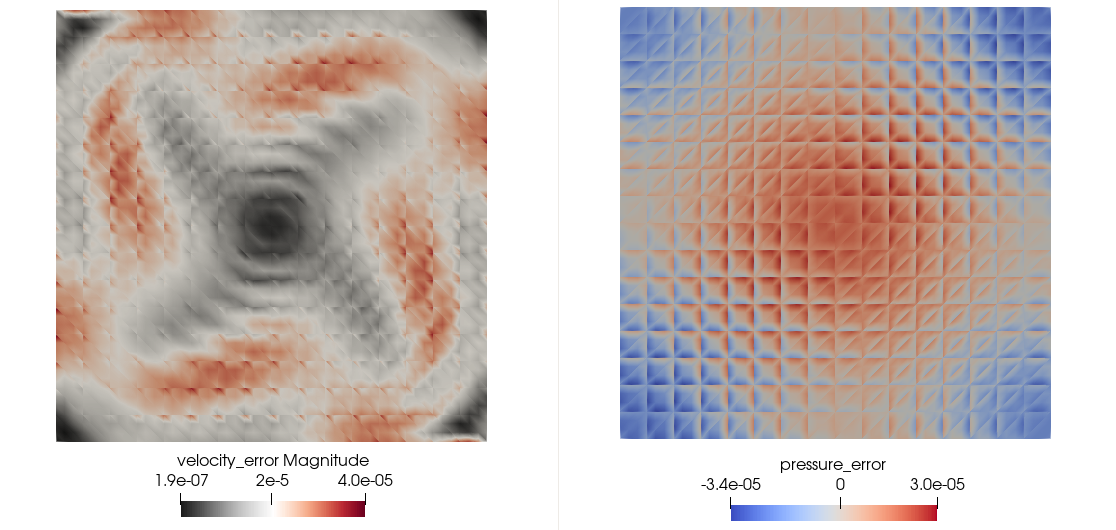
\includegraphics[width=1.0\linewidth]{figures/error_spatial.png}
        \caption{Spatial distribution of the error in velocity (left) and pressure (right) on a $16\times 16$ grid. Results are obtained with a SSP2(3,3,2) timestepper and a polynomial degree of $k=2$.}
        \label{fig:spatial_error}
    \end{center}
\end{figure}
To quantify convergence with this grid spacing $h$ we compute the $L_2$ error norm for increasing resolution. Fig. \ref{fig:L2error} shows how the error in the $L_2$ norm depends on the grid size for different polynomial degrees. For both velocity and pressure we observe convergence with the asymptotic rate  $\propto h^{k}\propto (\Delta t)^k$.
\begin{figure}
    \begin{center}
        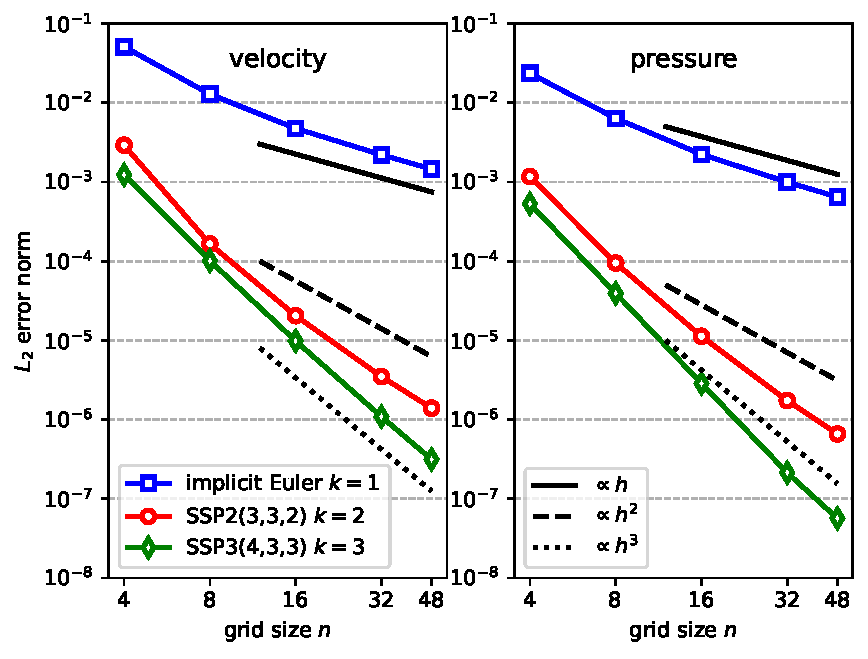
\includegraphics[width=0.75\linewidth]{figures/L2error.pdf}
        \caption{$L_2$ error norm in velocity (left) and pressure (right) for different grid sizes and polynomial degrees.}
        \label{fig:L2error}
    \end{center}
\end{figure}
%%%%%%%%%%%%%%%%%%%%%%%%%%%%%%%%%%%%%%%%%%%%%%%%%%%%%%%%%%%%%%%%%%%%%%%%%%%%%%%%%%%%%%%%%%%
\subsection{Performance}
%%%%%%%%%%%%%%%%%%%%%%%%%%%%%%%%%%%%%%%%%%%%%%%%%%%%%%%%%%%%%%%%%%%%%%%%%%%%%%%%%%%%%%%%%%%
Next, we investigate the performance of the different time integrators. For this, we first identify the computational bottlenecks.
%%%%%%%%%%%%%%%%%%%%%%%%%%%%%%%%%%%%%%%%%%%%%%%%%%%%%%%%%%%%%%%%%%%%%%%%%%%%%%%%%%%%%%%%%%%
\paragraph{Breakdown of time per iteration.}
%%%%%%%%%%%%%%%%%%%%%%%%%%%%%%%%%%%%%%%%%%%%%%%%%%%%%%%%%%%%%%%%%%%%%%%%%%%%%%%%%%%%%%%%%%%
Recall that an $s$-stage method with $n_R$ Richardson iterations requires $s-1$ projections of the velocity to the $\text{BDM}_{k+1}^0$ space, $n_R(s-1)$ solves for the tentative velocity and $n_R(s-1)+2$ mixed pressure solves. We expect these operations to dominate the total cost and this is confirmed by Fig. \ref{fig:titer_breakdown} which shows a breakdown of the runtime; more detailed results can be found in Tab. \ref{tab:time_per_iteration_breakdown}. Somewhat surprisingly, for higher orders the runtime is dominated by the BDM projection. \hl{Need to look at the BDM projection - we are probably not using the best solver here.}
\begin{figure}
    \begin{center}
        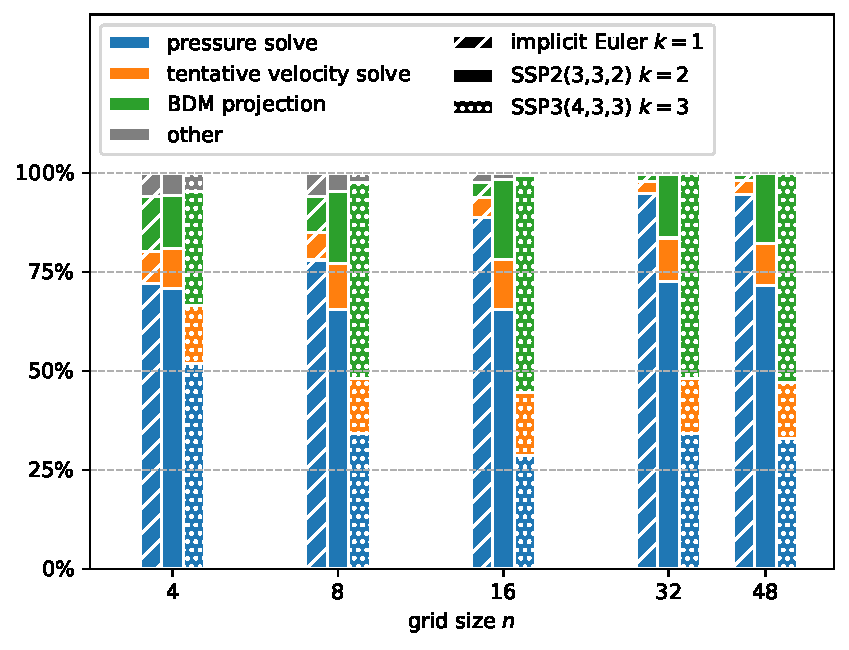
\includegraphics[width=0.75\linewidth]{figures/titer_breakdown.pdf}
        \caption{Fraction of runtime spent in the different solver components for varying grid size and different polynomial degrees.}
        \label{fig:titer_breakdown}
    \end{center}
\end{figure}
\begin{table}
    %%%%%%%%%%%%%%%%%%%%%%%%%%%%%%%%%%%%%%%%%%%%%%%%%%%%%%%%%%%%%%%%
\begin{center}
    implicit Euler, $k=1$\\[1ex]
    \begin{tabular}{|c|rcrcr|rcrcr|rcrcr|r|}
        \hline
        grid                                           &
        \multicolumn{5}{|c|}{pressure solve}           &
        \multicolumn{5}{|c|}{tentative velocity solve} &
        \multicolumn{5}{|c|}{BDM projection}           &
        timestep                                                                                                                                                           \\
        \hline\hline
        $ 4\times 4$                                   & 4 & $\times$ & 0.07 & $=$ & 0.28  & 2 & $\times$ & 0.01 & $=$ & 0.03 & 1 & $\times$ & 0.014 & $=$ & 0.014 & 0.34  \\
        $ 8\times 8$                                   & 4 & $\times$ & 0.06 & $=$ & 0.25  & 2 & $\times$ & 0.01 & $=$ & 0.02 & 1 & $\times$ & 0.008 & $=$ & 0.008 & 0.30  \\
        $16\times16$                                   & 4 & $\times$ & 0.17 & $=$ & 0.66  & 2 & $\times$ & 0.02 & $=$ & 0.04 & 1 & $\times$ & 0.005 & $=$ & 0.005 & 0.73  \\
        $32\times32$                                   & 4 & $\times$ & 1.01 & $=$ & 4.04  & 2 & $\times$ & 0.07 & $=$ & 0.14 & 1 & $\times$ & 0.004 & $=$ & 0.004 & 4.21  \\
        $64\times64$                                   & 4 & $\times$ & 4.17 & $=$ & 16.70 & 2 & $\times$ & 0.33 & $=$ & 0.65 & 1 & $\times$ & 0.004 & $=$ & 0.004 & 17.38 \\
        \hline\end{tabular}
\end{center}

%%%%%%%%%%%%%%%%%%%%%%%%%%%%%%%%%%%%%%%%%%%%%%%%%%%%%%%%%%%%%%%%
\begin{center}
    SSP2(3,3,2), $k=2$\\[1ex]
    \begin{tabular}{|c|rcrcr|rcrcr|rcrcr|r|}
        \hline
        grid                                           &
        \multicolumn{5}{|c|}{pressure solve}           &
        \multicolumn{5}{|c|}{tentative velocity solve} &
        \multicolumn{5}{|c|}{BDM projection}           &
        timestep                                                                                                                                                           \\
        \hline\hline
        $ 4\times 4$                                   & 6 & $\times$ & 0.06 & $=$ & 0.38  & 4 & $\times$ & 0.01 & $=$ & 0.06 & 2 & $\times$ & 0.008 & $=$ & 0.017 & 0.49  \\
        $ 8\times 8$                                   & 6 & $\times$ & 0.07 & $=$ & 0.40  & 4 & $\times$ & 0.02 & $=$ & 0.07 & 2 & $\times$ & 0.005 & $=$ & 0.010 & 0.50  \\
        $16\times16$                                   & 6 & $\times$ & 0.18 & $=$ & 1.08  & 4 & $\times$ & 0.05 & $=$ & 0.21 & 2 & $\times$ & 0.004 & $=$ & 0.007 & 1.34  \\
        $32\times32$                                   & 6 & $\times$ & 1.09 & $=$ & 6.53  & 4 & $\times$ & 0.25 & $=$ & 0.99 & 2 & $\times$ & 0.003 & $=$ & 0.006 & 7.56  \\
        $64\times64$                                   & 6 & $\times$ & 4.55 & $=$ & 27.32 & 4 & $\times$ & 1.04 & $=$ & 4.16 & 2 & $\times$ & 0.004 & $=$ & 0.009 & 31.54 \\
        \hline\end{tabular}
\end{center}

%%%%%%%%%%%%%%%%%%%%%%%%%%%%%%%%%%%%%%%%%%%%%%%%%%%%%%%%%%%%%%%%
\begin{center}
    SSP3(4,3,3), $k=3$\\[1ex]
    \begin{tabular}{|c|rcrcr|rcrcr|rcrcr|r|}
        \hline
        grid                                           &
        \multicolumn{5}{|c|}{pressure solve}           &
        \multicolumn{5}{|c|}{tentative velocity solve} &
        \multicolumn{5}{|c|}{BDM projection}           &
        timestep                                                                                                                                                            \\
        \hline\hline
        $ 4\times 4$                                   & 8 & $\times$ & 0.06 & $=$ & 0.46  & 6 & $\times$ & 0.02 & $=$ & 0.11  & 3 & $\times$ & 0.007 & $=$ & 0.020 & 0.62  \\
        $ 8\times 8$                                   & 8 & $\times$ & 0.07 & $=$ & 0.56  & 6 & $\times$ & 0.04 & $=$ & 0.21  & 3 & $\times$ & 0.004 & $=$ & 0.013 & 0.82  \\
        $16\times16$                                   & 8 & $\times$ & 0.21 & $=$ & 1.66  & 6 & $\times$ & 0.15 & $=$ & 0.91  & 3 & $\times$ & 0.003 & $=$ & 0.010 & 2.62  \\
        $32\times32$                                   & 8 & $\times$ & 1.19 & $=$ & 9.54  & 6 & $\times$ & 0.67 & $=$ & 4.02  & 3 & $\times$ & 0.004 & $=$ & 0.011 & 13.62 \\
        $64\times64$                                   & 8 & $\times$ & 4.92 & $=$ & 39.35 & 6 & $\times$ & 2.71 & $=$ & 16.26 & 3 & $\times$ & 0.007 & $=$ & 0.022 & 55.71 \\
        \hline\end{tabular}
\end{center}
    \begin{center}
        \caption{Breakdown of the time spent in the solver components for each timestep. For each component, the time per call and the number of calls per timestep is given. The total time per timestep is listed in the final column. Results are shown for the 2-stage implicit Euler method, the 3-stage SSP2(3,3,2) integrator and the 4-stage SSP3(4,3,3) timestepper.}
        \label{tab:time_per_iteration_breakdown}
    \end{center}
\end{table}
%%%%%%%%%%%%%%%%%%%%%%%%%%%%%%%%%%%%%%%%%%%%%%%%%%%%%%%%%%%%%%%%%%%%%%%%%%%%%%%%%%%%%%%%%%%
\paragraph{Robustness of the solvers.}
%%%%%%%%%%%%%%%%%%%%%%%%%%%%%%%%%%%%%%%%%%%%%%%%%%%%%%%%%%%%%%%%%%%%%%%%%%%%%%%%%%%%%%%%%%%
In the following we discuss the $h-$ and $p-$ robustness of the pressure- and tentative velocity solves \hl{Include BDM projection in analysis.}. Since both solves are performed with iterative methods, it is crucial to quantify the number of solver iterations that are required to achieve convergence. We manually set at relative tolerance of $10^{-12}$ on the preconditioned residual for the pressure solve and use the PETSc default setting for the tentative velocity solver. Fig. \ref{fig:niter} shows the average number of iterations\footnote{For the pressure solver, we only consider the final pressure solve in each timestep. However, we verified that the other solves require approximately the same number of iterations.} as a function of the grid size both for the tentative velocity solver and the pressure solver. The figure demonstrates that empirically both solvers are robust as the grid size $n$ and polynomial degree $k$ increases. Since (ideally) each solver iteration incurs a cost proportional to the number of unknowns, we therefore expect the cost of a single timestep to be proportial to number of unknowns for a given timestepper and polynomial degree $k$.
\begin{figure}
    \begin{center}
        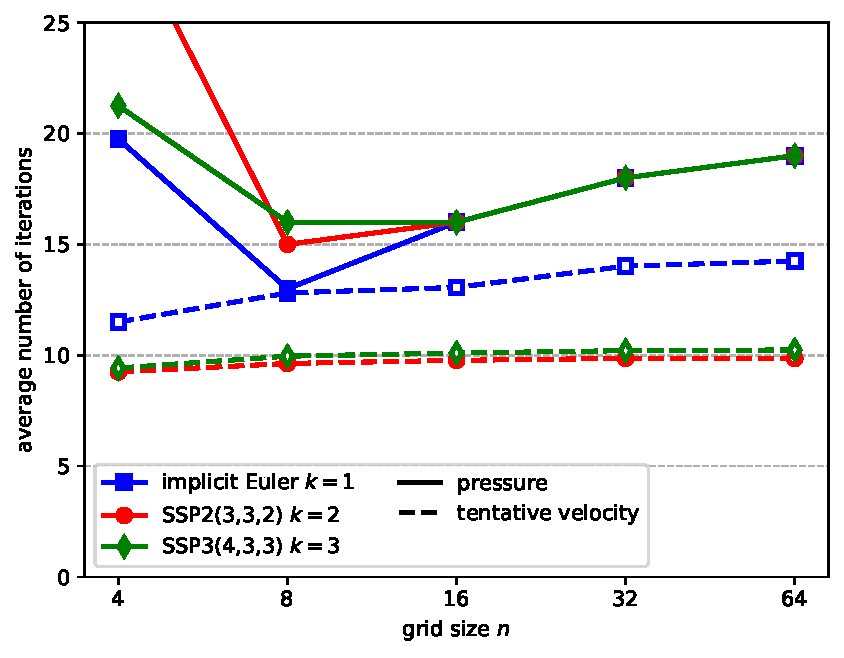
\includegraphics[width=0.75\linewidth]{figures/niter.pdf}
        \caption{Number of solver as a function of the grid size for different polynomial degrees.}
        \label{fig:niter}
    \end{center}
\end{figure}
This time per timestep is plotted as a function of the grid size for different polynomial degrees in Fig. \ref{fig:titer}. Naturally, this cost increases for higher polynomial degrees $k$. Asymptotically, for fixed $k$ the time per timestep grows in proportion to the number of unknowns, which is proportional to $n^2\propto h^{-2}$.
\begin{figure}
    \begin{center}
        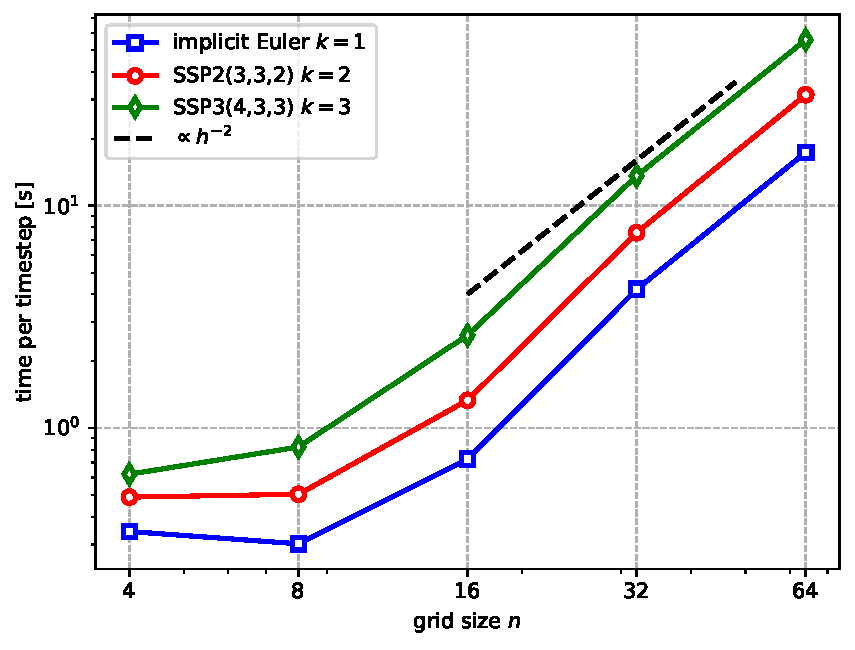
\includegraphics[width=0.75\linewidth]{figures/ttimestep.pdf}
        \caption{Time per timestep as a function of the grid size for different polynomial degrees.}
        \label{fig:titer}
    \end{center}
\end{figure}
%%%%%%%%%%%%%%%%%%%%%%%%%%%%%%%%%%%%%%%%%%%%%%%%%%%%%%%%%%%%%%%%%%%%%%%%%%%%%%%%%%%%%%%%%%%
\paragraph{Total runtime.}
%%%%%%%%%%%%%%%%%%%%%%%%%%%%%%%%%%%%%%%%%%%%%%%%%%%%%%%%%%%%%%%%%%%%%%%%%%%%%%%%%%%%%%%%%%%
The most useful metric to quantify the performance of a given setup is the total runtime for a given error. We plot this time as a function of both the $L_2$ velocity error norm and the $L_2$ pressure error norm in Fig. \ref{fig:ttotal}. For a fixed error budget higher order integrator have a significantly smaller overall runtime as the bound on the error decreases.
\begin{figure}
    \begin{center}
        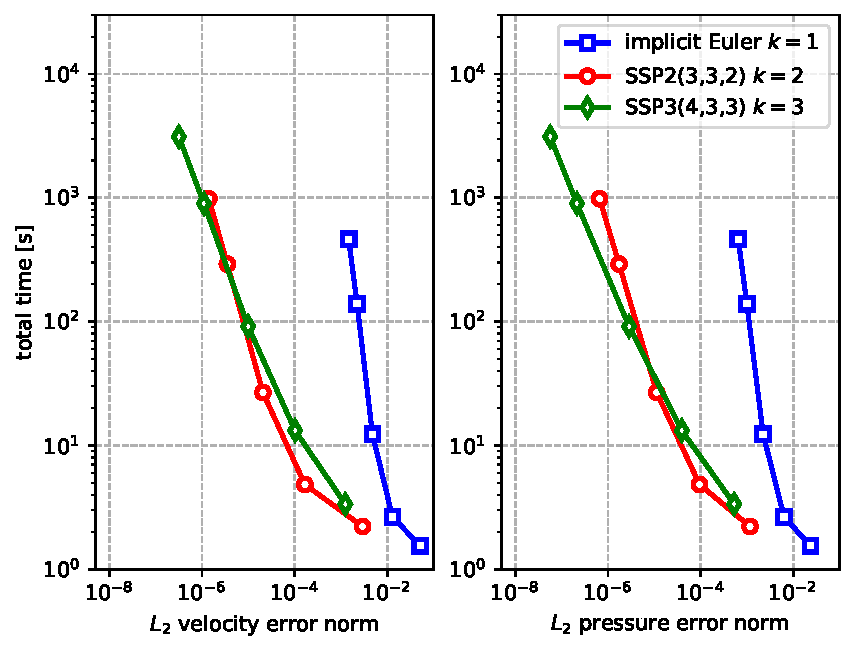
\includegraphics[width=0.75\linewidth]{figures/ttotal.pdf}
        \caption{Total runtime for different values of the $L_2$ error in velocity (left) and pressure (right).}
        \label{fig:ttotal}
    \end{center}
\end{figure}
\clearpage
%%%%%%%%%%%%%%%%%%%%%%%%%%%%%%%%%%%%%%%%%%%%%%%%%%%%%%%%%%%%%%%%%%%%%%%%%%%%%%%%%%%%%%%%%%%
\appendix
%%%%%%%%%%%%%%%%%%%%%%%%%%%%%%%%%%%%%%%%%%%%%%%%%%%%%%%%%%%%%%%%%%%%%%%%%%%%%%%%%%%%%%%%%%%
\section{Exact solution}\label{sec:exact_solution}
%%%%%%%%%%%%%%%%%%%%%%%%%%%%%%%%%%%%%%%%%%%%%%%%%%%%%%%%%%%%%%%%%%%%%%%%%%%%%%%%%%%%%%%%%%%
An exact solution of the two-dimensional incompressible Euler equations in Eq. \eqref{eqn:incompressible_euler} is given by for the stationary case $f=0$ by
\begin{equation}
    \begin{aligned}
        Q_s(x,y) & = \begin{pmatrix}-C(x)S(y)\\S(x)C(y)\end{pmatrix} \\
        p_s(x,y) & = p_0 - C(x)C(y)
    \end{aligned}
\end{equation}
where
\begin{xalignat}{2}
    S(z) &= \sin\left(\frac{2z-1}{2}\pi\right),&
    C(z) &= \cos\left(\frac{2z-1}{2}\pi\right).
\end{xalignat}
Note that the derivatives of these functions satisfy $S'(z)=\pi C(z)$ and $C'(z)=-\pi S(z)$. From this a divergence-free time-dependent solution for the special case
\begin{equation}
    f = \frac{d\Psi}{dt} Q_s(x,y).\label{eqn:forcing_exact}
\end{equation}
with arbitrary scalar function $\Psi(t)$ can be constructed as
\begin{xalignat}{2}
    Q(x,y,t) & = \Psi(t)Q_s(x,y),&
    p(x,y,t) & = \Psi(t)^2 p_s(x,y).\label{eqn:exact_solution}
\end{xalignat}
%%%%%%%%%%%%%%%%%%%%%%%%%%%%%%%%%%%%%%%%%%%%%%%%%%%%%%%%%%%%%%%%%%%%%%%%%%%%%%%%%%%%%%%%%%%
\bibliographystyle{unsrt}
\bibliography{discretisation}
\end{document}